\documentclass[10pt,a4paper]{article}

\usepackage[margin=1.5cm,top=1.2cm,bottom=1.2cm]{geometry}
\usepackage[T1]{fontenc}
\usepackage[utf8]{inputenc}
\usepackage{mathptmx}
\usepackage{amsmath,amssymb}
\usepackage{booktabs}
\usepackage{array}
\usepackage{enumitem}
\usepackage{xcolor}
\usepackage{fancyhdr}
\usepackage[nobottomtitles*]{titlesec}
\renewcommand{\bottomtitlespace}{0.04\textheight}
\titlespacing*{\section}{0pt}{7pt}{3pt}
\titleformat*{\section}{\normalsize\bfseries\color{navy}}
\usepackage[colorlinks=true,linkcolor=black,urlcolor=blue!60!black]{hyperref}
\usepackage{graphicx}
\usepackage[section]{placeins}  % figures and tables stay inside their own section
\usepackage{listings}
\lstset{language=Python, basicstyle=\ttfamily\footnotesize, columns=fullflexible, keepspaces=true,
        commentstyle=\color{gray!70!black}, keywordstyle=\color{navy}, frame=single,
        rulecolor=\color{gray!40}, xleftmargin=4pt, xrightmargin=4pt, aboveskip=4pt, belowskip=2pt}

% generated by plot_results.py from results/population_recovery_*.json; do not edit by hand
\newcommand{\popRandomStarts}{20}
\newcommand{\popMaxIterations}{2000}
\newcommand{\popCellsSmall}{300}
\newcommand{\popLlTrueSmall}{-4026.23}
\newcommand{\popLlBestSmall}{-4018.00}
\newcommand{\popLlHouseholderSmall}{-4022.48}
\newcommand{\popStartsAtBestSmall}{2}
\newcommand{\popFirstStartAtBestSmall}{4}
\newcommand{\popBestStartSmall}{10}
\newcommand{\popErrMASmall}{0.05}
\newcommand{\popErrTSmall}{0.21}
\newcommand{\popErrMUSmall}{0.05}
\newcommand{\popErrPiSmall}{0.04}
\newcommand{\popErrMeansSmall}{0.31}
\newcommand{\popErrHouseholderSmall}{0.97}
\newcommand{\popProportionGapSmall}{0.024}
\newcommand{\popCellsLarge}{3000}
\newcommand{\popLlTrueLarge}{-39870.38}
\newcommand{\popLlBestLarge}{-39863.19}
\newcommand{\popLlHouseholderLarge}{-39937.96}
\newcommand{\popStartsAtBestLarge}{5}
\newcommand{\popFirstStartAtBestLarge}{10}
\newcommand{\popBestStartLarge}{19}
\newcommand{\popErrMALarge}{0.04}
\newcommand{\popErrTLarge}{0.13}
\newcommand{\popErrMULarge}{0.05}
\newcommand{\popErrPiLarge}{0.02}
\newcommand{\popErrMeansLarge}{0.15}
\newcommand{\popErrHouseholderLarge}{0.85}
\newcommand{\popProportionGapLarge}{0.002}
  % numbers quoted in the text, generated by plot_results.py from results/*.json

% ---------- Report information (edit here) ----------
\newcommand{\myname}{Arnab Kumar Ghosh}
\newcommand{\reporttitle}{Progress Report}
\newcommand{\projecttitle}{Discrete State-Space Models and Expectation-Maximization for Cell-State Trajectories}
\newcommand{\supervisor}{Prashant Singh}
\newcommand{\period}{Weeks 7--8}
\newcommand{\reportdate}{\today}
% ----------------------------------------------------

% Draft marker: things to check before sending. Remove the marker once checked.
\newcommand{\tocheck}[1]{\textcolor{red}{[#1]}}

\definecolor{navy}{RGB}{31,56,100}
\setlist{nosep, leftmargin=1.4em}
\setlength{\parskip}{2pt}
\AtBeginDocument{\setlength{\abovedisplayskip}{4pt}\setlength{\belowdisplayskip}{4pt}}
\setlength{\parindent}{0pt}

\pagestyle{fancy}
\fancyhf{}
\rhead{\small Progress report -- \period}
\cfoot{\small\thepage}
\renewcommand{\headrulewidth}{0.3pt}

\newcommand{\sub}[1]{\vspace{1pt}\textbf{\textcolor{gray!80!black}{#1}}\par}

\begin{document}

% ---------- Title block ----------
\begin{center}
  {\Large\bfseries\textcolor{navy}{\reporttitle}}\\[2pt]
  {\projecttitle}\\[3pt]
  {\small \myname\ \textperiodcentered\ Supervisor: \supervisor\ \textperiodcentered\ MSc Computer Science, Uppsala University \textperiodcentered\ \period\ \textperiodcentered\ \reportdate}
\end{center}
\vspace{-2pt}
\hrule
\vspace{4pt}

% ---------- 0. Overview ----------
\section*{Overview}
In weeks 7--8 I implemented the population model and its EM algorithm, and tested them on simulated cells from the 2D toy model of the last report.
\begin{itemize}
  \item The code matches the hand-check values, and $\ell$ never decreases during EM.
  \item On simulated cells the MA and MU rows of $A$ are recovered well, the T row worst.
  \item EM often stops at a lower $\ell$ (a local maximum), so I fit from 21 starts and keep the fit with the highest $\ell$.
\end{itemize}

Done from the plan of the last report:
\begin{enumerate}
  \item Implement the 2D toy population model and pass the hand-check values (Section 1).
  \item Run the recovery experiment on the 2D toy (Sections 2--3).
\end{enumerate}
The rest of that plan (the day-0 experiment, the 5D toy and the first look at the real data) is in the plan for the next two weeks (Section 4).

% ---------- 1 ----------
\section{Implementation and checks}

The model and EM are in \texttt{population\_model.py}, the starting values in \texttt{starting\_values.py}, and the true toy parameters in \texttt{toy\_parameters.py}. The code is in the GitHub repository \url{https://github.com/bdtiger/open-course-on-topics} (folder \texttt{project-code}). The fitting code gets only the expression matrix $X$ (one row per cell, one column per gene) and the week of each cell. For simulated cells, the true state of each cell is kept aside and used only to compare afterwards. So the same code can run on the real data.

One fix was needed: in the $\pi$, $A$ step a probability could round to exactly 0 in floating point, and after that $\pi$ and $A$ stopped changing. Every entry of $\pi$ and $A$ is now kept at $10^{-10}$ or above.

The checks in \texttt{checks.py} all pass (Table~\ref{tab:checks}). Two of them cannot expect exact equality, so they pass if the gap stays below a limit I chose. For the simulator, random sampling never matches the parameters exactly; the limits are 0.02 for the state fractions and 0.1 for the means and variances, a few times the random error expected with 3000 cells per week and much smaller than the error a bug would cause. For the $\pi$, $A$ step, the numerical optimiser stops close to the optimum but not exactly on it; the limit is $10^{-3}$. The table gives the actual gaps.

\begin{table}[!htb]
\centering
\small
\begin{tabular}{@{}lll@{}}
\toprule
Check & Compared with & Result \\
\midrule
Proportions $p_1, p_2, p_3$ & hand values & equal \\
Simulator, 3000 cells per week & $p_t$, $\mu_j$, $\sigma^2_j$ & largest gap: fractions 0.009, means and variances 0.02 \\
$\log \mathcal{N}$, $r$ and $\ell$ of the four hand-check cells & hand values & equal to 4 decimals \\
One Gaussian update from the hand-check cells & hand values & equal to 4 decimals \\
$\pi$, $A$ step with exact proportions $n_t = 10^5\, p_t$ & true $\pi$, $A$ & largest gap $2 \times 10^{-7}$ \\
State matching on the 6 reorderings of the true parameters & true order & order restored exactly \\
EM (every iteration) & previous $\ell$ & $\ell$ never decreases \\
\bottomrule
\end{tabular}
\caption{Checks of the implementation. Hand values are from the hand-check sheet of the last report.}
\label{tab:checks}
\end{table}

% ---------- 2 ----------
\section{Several starts}

\sub{What I found}
EM only climbs: every iteration raises $\ell$, and it stops when $\ell$ no longer rises. Where it stops depends on where it starts, and from many starts it stops at a lower $\ell$ (a local maximum). For example, two states can share the MA cells while no state covers T.

I therefore fit from 21 starts and keep the fit with the highest final $\ell$:
\begin{itemize}
  \item the Householder start from the last report (k-means means and variances, $A$ from the Householder formula);
  \item \popRandomStarts{} random starts (random $\pi$ and $A$, three random cells as the means, the variance of all cells as the variances).
\end{itemize}

Figure~\ref{fig:loglik} shows $\ell$ for every start. Only \popStartsAtBestSmall{} of the 21 starts at \popCellsSmall{} cells per week, and \popStartsAtBestLarge{} of 21 at \popCellsLarge{}, reach the best $\ell$ (within 0.1). The Householder start does not reach it at either size. At \popCellsLarge{} cells per week the first random start that reaches it is number \popFirstStartAtBestLarge{}, so the five random starts I had planned would have missed it. Some starts stay flat for hundreds of iterations before they climb again (blue line, left), so I allow up to \popMaxIterations{} iterations per start; one start at \popCellsSmall{} cells per week was still climbing slowly when it reached this limit.

\begin{figure}[!htb]
\centering
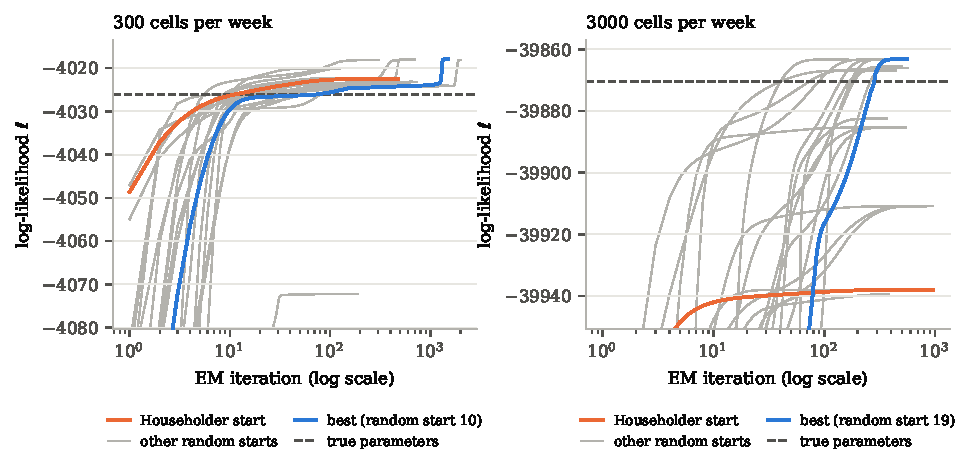
\includegraphics[width=\textwidth]{figures/population_log_likelihood.pdf}
\caption{$\ell$ per EM iteration for every start (iteration axis logarithmic). Blue: the start with the highest final $\ell$. Orange: the Householder start. Gray: the other random starts; each flat end is a local maximum. Dashed: $\ell$ of the true parameters.}
\label{fig:loglik}
\end{figure}

\sub{In the project}
On the real data there is no true answer to compare with, so fits can only be compared by $\ell$. I will run many random starts, keep the best $\ell$, and report how many starts reach it.

% ---------- 3 ----------
\section{Recovery of the true parameters}

\sub{What I did}
I simulated \popCellsSmall{} and \popCellsLarge{} cells per week for the four weeks from the true toy parameters (Figure~\ref{fig:cells}), fitted them as in Section 2, and compared the best fit with the true parameters. EM numbers its states in no particular order, so before comparing I name each fitted state after the true state with the closest mean.

\begin{figure}[!htb]
\centering
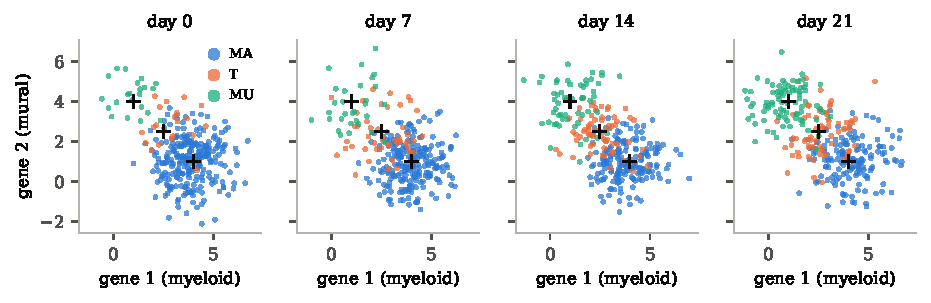
\includegraphics[width=\textwidth]{figures/population_cells_300.pdf}
\caption{Simulated cells, \popCellsSmall{} per week, coloured by their true state (the fit never sees the states). Crosses: true means. Over the weeks the population moves from MA towards T and MU.}
\label{fig:cells}
\end{figure}

\sub{What I found}
Figure~\ref{fig:A} shows the results.
\begin{itemize}
  \item The MA and MU rows of $A$ are recovered well, the T row worst. The largest error $|\text{fitted} - \text{true}|$ in each row is \popErrMASmall{} (MA), \popErrTSmall{} (T) and \popErrMUSmall{} (MU) at \popCellsSmall{} cells per week, and \popErrMALarge, \popErrTLarge{} and \popErrMULarge{} at \popCellsLarge. More cells improve the MA and T rows; the MU row has the same error at both sizes.
  \item The last report (Section 6) predicted the T and MU rows to be less accurate than the MA row. This holds for T but not for MU.
  \item The best fit has a slightly higher $\ell$ than the true parameters at both sizes ($\popLlBestSmall$ against $\popLlTrueSmall$ at \popCellsSmall{} cells per week, $\popLlBestLarge$ against $\popLlTrueLarge$ at \popCellsLarge). This is expected: the fit also adapts to the random noise in this particular sample of cells.
\end{itemize}

\begin{figure}[!htb]
\centering
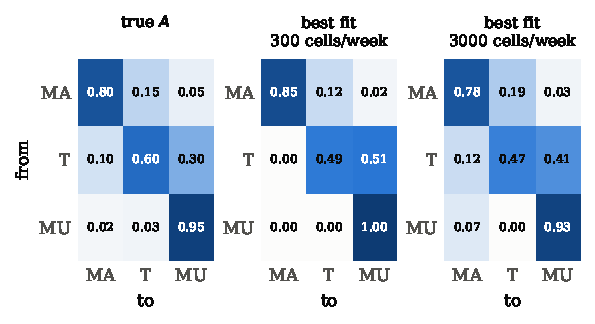
\includegraphics[width=0.6\textwidth]{figures/population_transition_matrices_best.pdf}
\caption{True $A$ and the $A$ of the best fit at \popCellsSmall{} and \popCellsLarge{} cells per week. Rows: from; columns: to. Each fitted state is named after the true state with the closest mean.}
\label{fig:A}
\end{figure}

\sub{In the project}
On the real data I expect the T row to be the least certain. Before I interpret it, I will report how much each row of $A$ changes across starts and resampled cells, as planned in the last report.

% ---------- 4 ----------
\section{Plan for the next two weeks}

\begin{enumerate}
  \item Finish the toy experiments:
  \begin{itemize}
    \item Day-0 experiment: refit the simulated cells without the day-0 cells, from several starts, to check that $A$ cannot be estimated without the healthy cells (expected: different starts end at different $A$ with almost the same $\ell$).
    \item Test set: keep 20\% of the cells aside from fitting, and compare their $\ell$ under the best fit with their $\ell$ under the true parameters.
    \item The 5D toy with one gene that carries no signal.
  \end{itemize}
  \item Real data, first look only: open \texttt{adata\_final.h5ad}, select the 50 genes, check the normalisation, and count the cells per day, batch and cluster, before any fitting.
\end{enumerate}

\end{document}
